\section{Pré-étude} \label{sec:Pre-Etude}

\subsection{Fonctionnement du système} \label{ssec:Fonctionnement}
Le microcontrôleur interagît avec 4 périphériques principaux : Avec le \gls{GNSS}, il partage une communication qui lui permet d'obtenir les informations de localisation par le biais de plusieurs systèmes de satellites. Il y a ensuite, la centrale inertielle qui lui donne accès de une multitude de mesures sur 9 axes, or, ici les mesures gyroscopiques et d'accélération sont exploitées. La carte SD, permet quant-à-elle, de stocker toutes ces données pour avoir minimum les information des 15 dernières minutes de vol. Le dernier périphériques principale \gls{FTDI}, permet d'avoir une interface avec un ordinateur via connexion USB-C.

\subsection{Schéma bloc} \label{ssec:Schema-bloc}

\begin{figure}[h]
	\centering
	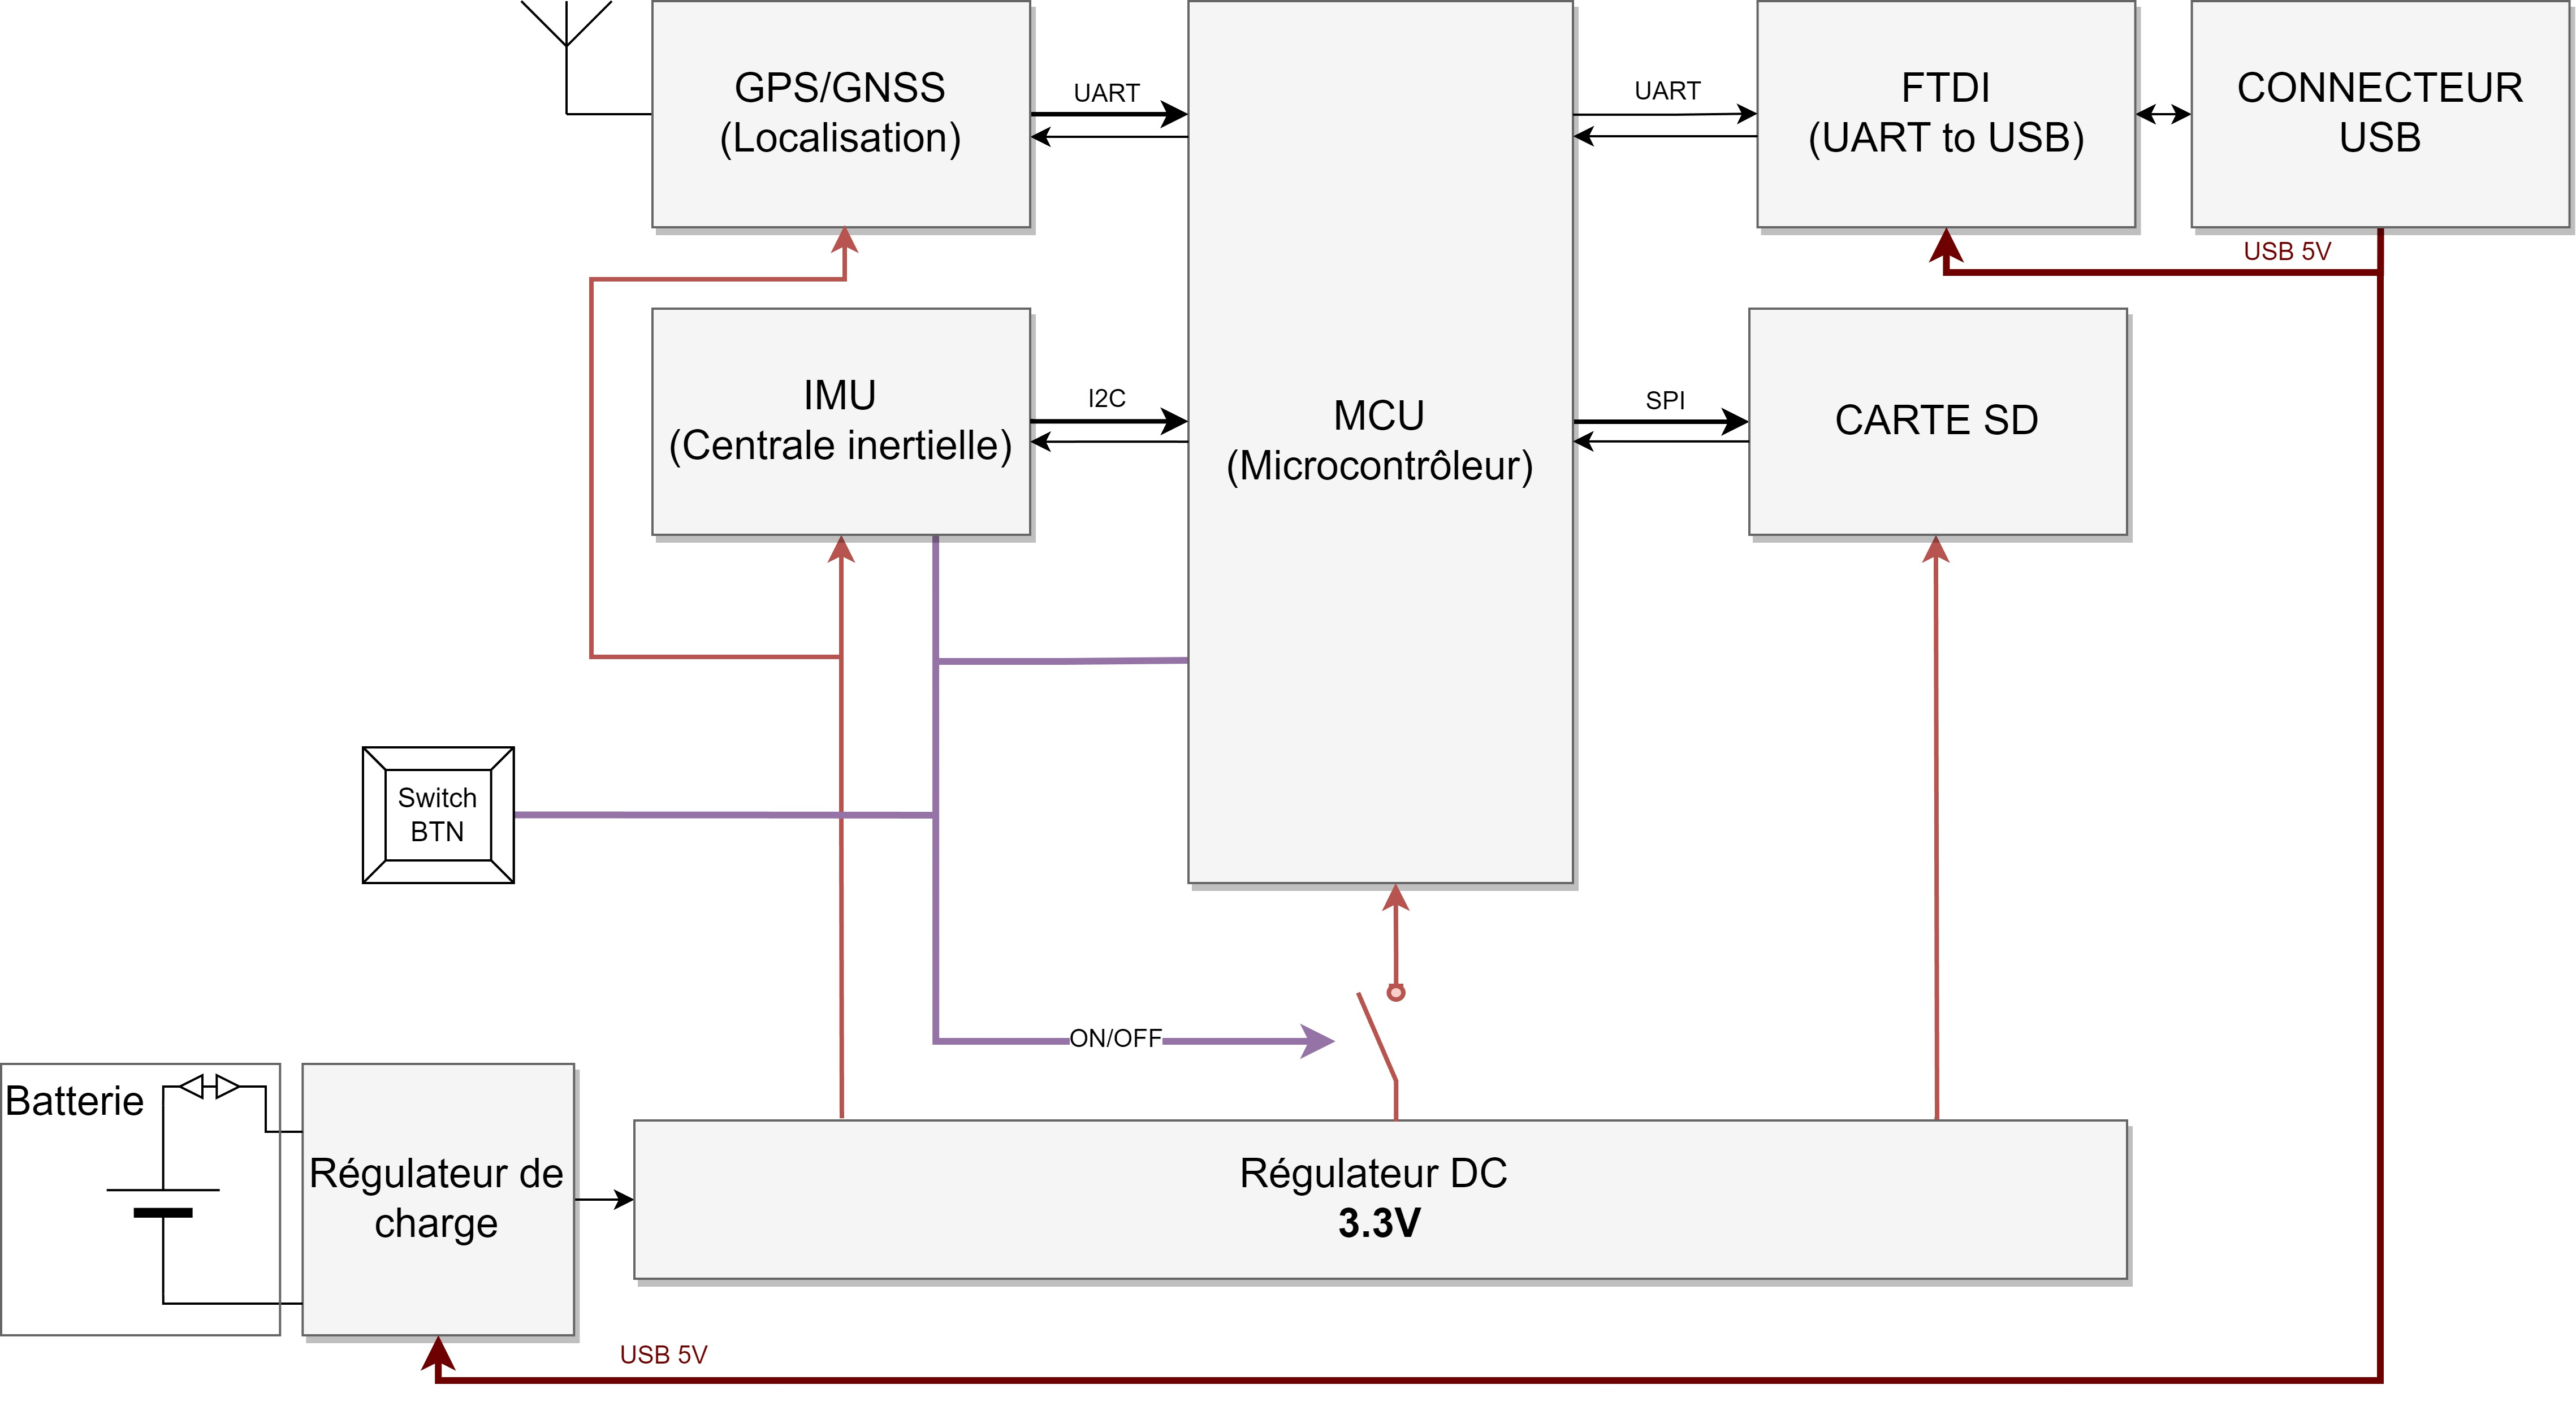
\includegraphics[width=1\textwidth]{../figures/cdc/blocs_grossiers_no_antenna.jpg}
	\caption{Schéma bloc}
	\label{fig:schbloc}
	\source{Auteur}
\end{figure}
% ---- Description des blocs ----
\subsection{Description des blocs} \label{ssec:Desc-blocs}

\begin{table}[h]
	\resizebox{\columnwidth}{!}{%
		\begin{tabular}{|l|l|}
			\hline
			Bloc         & Description                                                                         \\ \hline
			\Gls{gnss}.  & Récepteur \Gls{rf} avec antenne interne/externe et communication UART.              \\ \hline
			\Gls{mcu}.   & Microcontrôleur PIC32, intelligence du système, basse consommation.                 \\ \hline
			\Gls{imu}.   & Centrale inertielle, accélération, gyroscope...                                     \\ \hline
			Carte SD     & Stockage des données de vol.                                                        \\ \hline
			\Gls{FTDI}.  & Convertis la communication USB en série.                                            \\ \hline
			Régulateurs. & Le régulateur de charge gère la charge de l'accu. et un régulateur 3.3V le suit.    \\ \hline
			Batterie.    & La batterie est un accu que l'on peut charger par USB et permet une bonne autonomie. \\ \hline
		\end{tabular}%
	}
\end{table}

\clearpage
\raggedbottom
\subsection{Choix des composants et technologies} \label{sssec:ComposantsTech}
L'objectif de la pré-étude consiste en grande partie à sélectionner méthodiquement les technologies et les composants du projet. Cette partie du travail est essentielle et critique.

\subsubsection{Microcontrôleur}
Le microcontrôleur nécessite au minimum les périphériques suivants : \\
\fbox{2 UART} \fbox{1 SPI} \fbox{1 I2C} \\
Il est préférable que le \gls{mcu} dispose de différentes configurations de gestion de puissance, notamment des modes d'économie d'énergie, afin d'avoir une maîtrise de la consommation et de permettre une meilleure autonomie. Enfin, le standard de l'école veut que les familles de microcontrôleurs PIC32 (Microchip) sont préférées.

\begin{figure}[h]
	\centering
	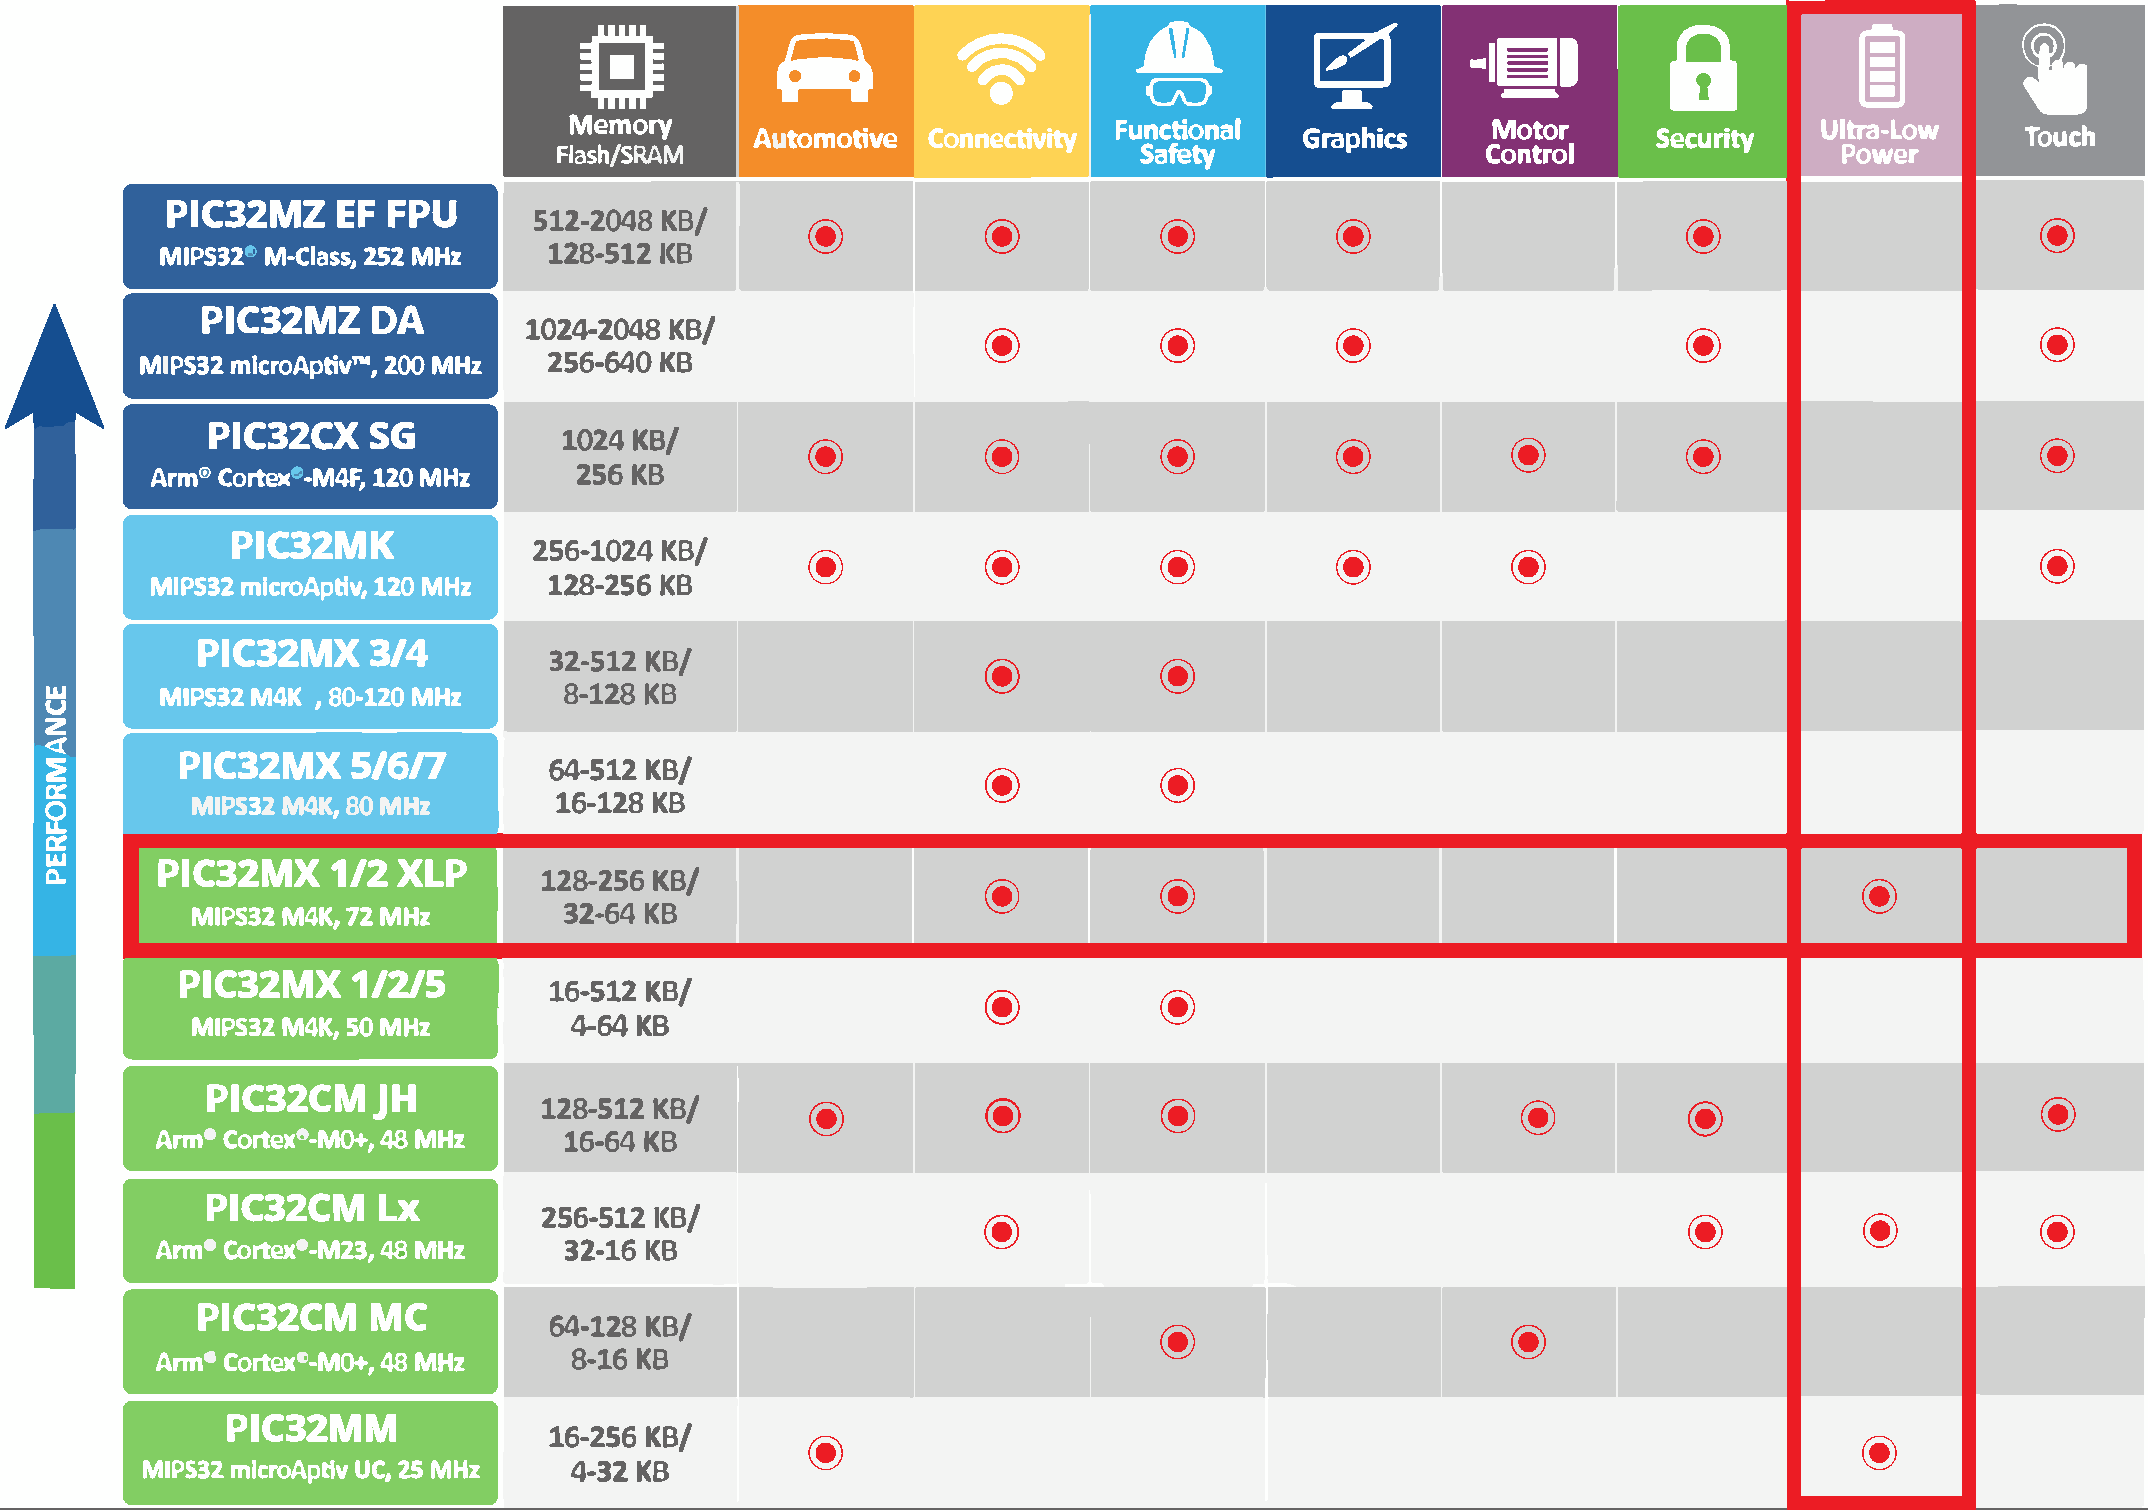
\includegraphics[width=0.65\linewidth]{../figures/pre_etude/familles_pic32}
	\caption{Familles PIC32}
	\label{fig:famillespic32}
	\source{\href{https://www.microchip.com/en-us/products/microcontrollers-and-microprocessors/32-bit-mcus/pic32-32-bit-mcus}{https://www.microchip.com/en-us/products/microcontrollers-and-microprocessors/32-bit-mcus/pic32-32-bit-mcus}}
\end{figure}

Sur la figure \ref{fig:famillespic32} le \gls{mcu} sélectionné appartient à la gamme MX (Baseline performance-mémoire) et à la famille XLP qui offre notamment la fonctionnalité "Ultra low power" qui est celle qui nous intéresse.

\begin{figure}[h]
	\centering
	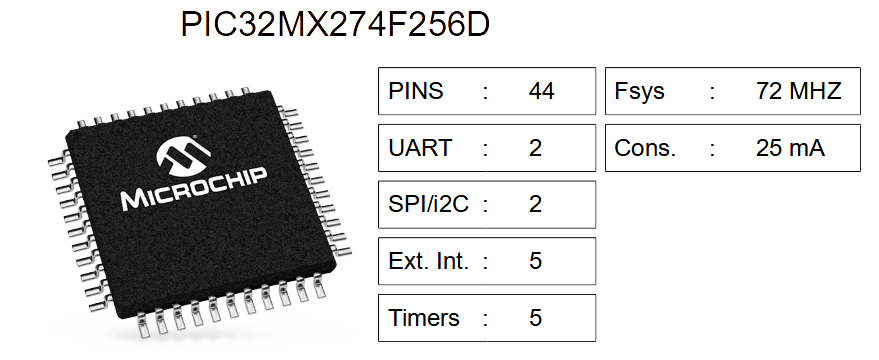
\includegraphics[width=0.7\linewidth]{../figures/pre_etude/Carac_PIC32}
	\caption{Caractéristiques du PIC32 choisi}
	\source{Auteur}
	\label{fig:caracpic32}
\end{figure}

\clearpage
\subsubsection{Centrale inertielle} 
Pour la centrale inertielle, il existe un composant avec lequel j'ai déjà acquis une certaine expérience et eu l'occasion d'utiliser et de créer des librairies pour le firmware en C. Celui-ci est performant et très utilisé dans l'industrie. Il est hautement configurable et a le grand avantage de calculer déjà une fusion de capteurs ainsi qu'une compensation de la dérive par les mesures de température. Cela permet notamment d'accéder à des données plus poussées, telles que les quaternions et les angles d'Euler. Il s'agit du \fbox{BNO055} de BOSCH.
 
\begin{center}
	\underline{Caractéristiques importantes :} \\
	\begin{tabular}{l l l l}
		Résolution gyroscope & : & 16 & [bits] \\
		Résolution accéléromètre & : & 14 & [bits] \\
		Résolution magnétomètre & : & $\sim$0.3 & [$\mu$T] \\
		$I_{DD}$ & : & 12.3 & [mA] \\
		Dérive de température & : & $\pm$ 0.03 & [\%/K] \\ 
		Dérive accéléromètre & : & 0.2 & [\%/V] \\
		Dérive gyroscope & : & <0.4 & [\%/V]
	\end{tabular} \\
\end{center}

Afin de simplifier l'implémentation de ce composant dans le projet, sachant qu'il s'agit d'un boîtier de composant difficile à souder ou à mettre au four, il est possible d'utiliser la carte miniature d'Adafruit, cette carte comprend tous les composants passifs requis. Cela facilite ainsi son montage sur le PCB.

\begin{figure}[h]
	\centering
	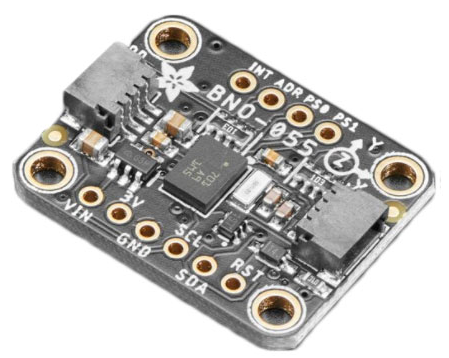
\includegraphics[width=0.45\linewidth]{../figures/pre_etude/BNO055_Adafruit}
	\caption{Carte d'extension, centrale inertielle}
	\source{\href{https://www.digikey.ch/en/products/detail/adafruit-industries-llc/4646/12609996?s=N4IgTCBcDaIEYDsD2AGArGgBAQwCbYDMAnAVwEsAXEAXQF8g}{Digikey, 4646}}
	\label{fig:bno055adafruit}
\end{figure}

\underline{Données disponibles :}

\begin{center}
	\begin{tabular}{|ll|}
		\hline
		Température & \\
		\hline
		Vecteur gravité & XYZ \\
		\hline
		Orientation compensées, quaternion & WXYZ \\
		\hline
		Orientation compensée, angle de Euler & HPR \\
		\hline
		Données gyroscopiques & XYZ \\
		\hline
		 Intensité du champ magnétique & XYZ \\
		\hline
		Accélération & XYZ \\
		\hline
	\end{tabular}
\end{center}

\clearpage

\subsubsection{GPS / GNSS}
Pour le \gls{GPS}/\gls{GNSS}, différents critères entrent en jeu dans le cadre de ce projet : le prix, la facilité d'implémentation, la complexité (par complexité, nous entendons le nombre de fonctionnalités), la consommation et la performance.

Il existe un très grand nombre de récepteurs \gls{rf} pour la navigation. Parmi les plus utilisés dans l'industrie, dont l'implémentation est la plus simple et la documentation la plus complète, il y a plusieurs gammes chez le fabricant \fbox{ublox}.
Deux composants ont principalement été pris en considération :
Le \textbf{CAM-M8C-0} (BeiDou, GLONASS, GNSS, GPS, QZSS) avec une antenne omnidirectionnelle interne au composant et différents modes de puissance, ainsi que le \textbf{MAX-M10M-00B} (BeiDou, Galileo, GLONASS, GNSS, GPS) sans antenne interne mais avec une consommation de base plus faible.

\begin{figure}[h]
	\centering
	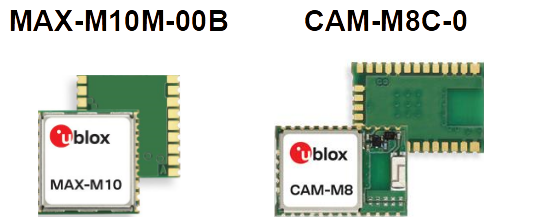
\includegraphics[width=0.6\linewidth]{../figures/pre_etude/img_gnss}
	\caption{Illustration des deux GNSS}
	\source{\href{https://www.digikey.ch/fr/products/detail/u-blox/CAM-M8C-0/6150647?s=N4IgTCBcDaIMIEECyBaJAOOKAMIC6AvkA}{Digikey}}
	\label{fig:imggnss}
\end{figure}


\begin{figure}[h]
	\centering
	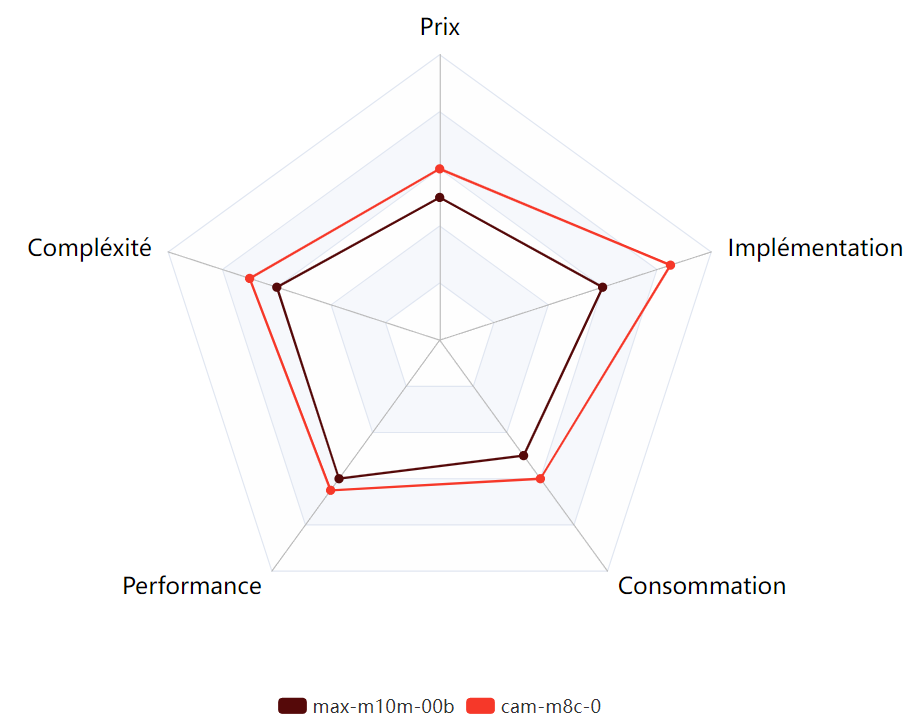
\includegraphics[width=0.65\linewidth]{../figures/pre_etude/Comp_GNSS}
	\caption{Comparaison GNSS}
	\source{Auteur}
	\label{fig:compgnss}
\end{figure}

Malgré les différents avantages que présente le MAX-M10M-00B sur la figure \ref{fig:compgnss}, le choix s'est porté sur CAM-M8C-0 grâce à sa facilitée d'implémentation et à la garantie du fabricant sur son antenne omnidirectionnelle de qualité.

\clearpage

\subsubsection{Carte SD} 
Les pilotes de carte SD disponibles dans \gls{harmony} ne permettent pas une gestion des capacités de stockage trop importantes. Cela signifie, que nous ne pouvons pas avoir des cartes SD de trop grandes capacités, c'est pour cela que nous allons baser nos dimensionnements sur une carte de \textbf{256MB}. 

\begin{figure}[h]
	\centering
	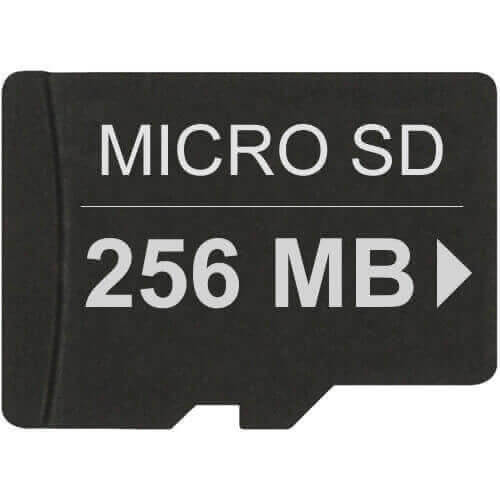
\includegraphics[width=0.2\linewidth]{../figures/pre_etude/CarteSD_Illustration}
	\caption{Illustration carte SD}
	\source{\href{https://www.oempcworld.com/OEMPCworld-com/017045.html}{https://www.oempcworld.com/OEMPCworld-com/017045.html}}
	\label{fig:cartesdillustration}
\end{figure}


\paragraph{Estimation de la capacité} Admettons les paramètres suivants où $S$ représente une taille de données et $T$ un temps :

\begin{tabular}{lrl}
	$S_{SD}$ & $256$ & $[KB]$ \\
	$S_{gyro}$ & $16$ & $[Bytes]$ \\
	$S_{accel}$ & $16$ & $[Bytes]$ \\
	$S_{gnss}$ & $\sim100$ & $[Bytes]$ \\
	$T_{inertiel}$ & $0.5$ & $[s]$ \\
	$T_{gnss}$ & $5$ & $[s]$ \\
	$T_{mesMin}$ & $900$ & $[s]$ \\
\end{tabular}

Nous pouvons déduire la taille mémoire que prendra 5 secondes d'enregistrement avec les paramètres par défaut du système : 
\begin{equation*}
	S_{single} = \frac{T_{gnss}}{T_{inertiel}}(S_{gyro}+S_{accel}) + S_{gnss} = \frac{5}{0.5}(16+16) + 100 = 420 \; [Bytes]
\end{equation*}

Nous pouvons enfin calculer à partir de cela, la taille mémoire que prendra 15 minutes d'enregistrement : 

\begin{equation*}
	S_{mesures} = \frac{S_{single}}{T_{gnss}} * T_{mesMin} = \frac{420}{5} * 900 = 75'600 \; [Bytes] = 75.6 \; [KB]
\end{equation*}

Nous pouvons déduire avec cette estimation qu'une carte SD de 256MB est largement suffisante et permet de mesurer jusqu'à un temps calculable de cette façon :

\begin{equation*}
	T_{mesures} = \frac{S_{SD}*T_{gnss}}{S_{single}} = \frac{256'000*5}{420} = \sim508 \; Minutes = \sim8.5 \; Heures
\end{equation*}

Nous estimons donc, que les données de vol des 8.5 dernières heures sont enregistrées dans la carte SD.

\clearpage

\subsubsection{Batterie, charge et régulation} 
Afin de dimensionner une batterie pour le projet, il faut considérer les différentes consommation :

\begin{center}
	\underline{Liste des consommations principales} \\
	\begin{tabular}{lrll}
		Microcontrôleur & 24 & [mA] & Typ. \\
		Carte-SD & ~100 & [mA] & Max. \\
		Carte-SD & ~60 & [mA] & Moyenne \\
		\gls{imu} & 12.3 & [mA] & Typ. \\
		\gls{GNSS} & 71 & [mA] & Max. \\
		\gls{GNSS} & 29 & [mA] & Typ. \\
		\hline
		Totale max & \underline{207.3} & [mA] & Max. \\
		Totale moyennes & \underline{125.3} & [mA] & Moyenne \\
		\hline
	\end{tabular}
\end{center}



En prenant les consommations 


\subsection{Systèmes d'économies d'énergie} \label{ssec:Low-power}
Dans le but de maximiser le temps de logging, des mécanismes d'économies d'énergie doivent être mis en place. 

\subsection{Estimation des coûts} \label{ssec:Estimation-Couts}
